\section{Tree Predictors}

\subsection{Definizione}
Come già visto, mentre alcuni tipi di dato hanno una naturale rappresentazione
vettoriale $x \in \RN^d$, altri non ce l'hanno. Un esempio possono essere dei
\textit{record} medici, dove i dati contengono i seguenti campi:
$$ \begin{aligned}
    &\texttt{età} \in \{12,\dots,90\} \\
    &\texttt{fumatore} \in \{\text{sì},\text{no},\text{ex}\} \\
    &\texttt{peso} \in [10,200] \\
    &\texttt{sesso} \in \{\text{M},\text{F}\} \\
    &\texttt{terapia} \in \{\text{antibiotici},\text{cortisone},\text{nessuna}\} \\
\end{aligned} $$

Anche convertendo questi tipi di dato in dati numerici, gli algoritmi basati sulla
distanza euclidea, come il \kNN, potrebbero non andare molto bene.

\textbf{Per poter applicare la \textit{data inference} su dati le cui 
\textit{feature} variano in insiemi eterogenei $\X_1,\dots,\X_d$, verrà introdotta 
una nuova famiglia di predittori: i \textit{tree predictors}}.

Un \textit{tree predictor} è un albero ordinato e radicato dove ogni nodo può
essere una \textbf{foglia} o un \textbf{nodo interno}. È importante sottolineare che
in un albero ordinato i figli di ogni nodo sono anch'essi ordinati e quindi numerabili
consecutivamente.
In figura \ref{fig:tree_class}
viene mostrato un esempio di \textit{tree predictor} binario le cui \textit{feature}
sono:
$$ \begin{aligned}
    &\texttt{previsione} \in \{\text{sole},\text{nuvole},\text{pioggia}\} \\
    &\texttt{umidità} \in [0,100] \\
    &\texttt{vento} \in \{\text{sì},\text{no}\}
\end{aligned} $$
 
\begin{figure}[h]
    \centering
    \usetikzlibrary {shapes.geometric}
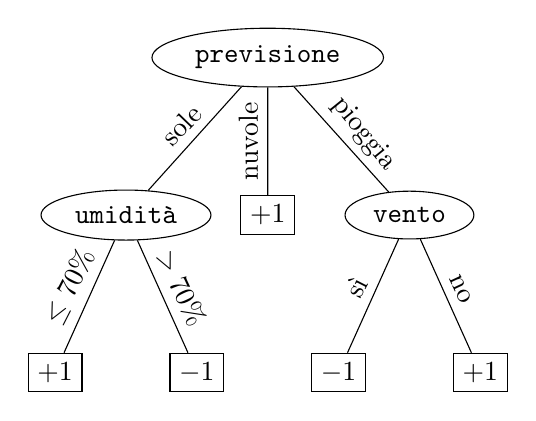
\begin{tikzpicture}[sibling distance=18mm, level distance=20mm]
    
    \node [ellipse,draw] {\texttt{previsione}}
        child {node[ellipse,draw] {\texttt{umidità}}
            child {node[rectangle,draw] {$+1$} edge from parent node[above,rotate=63] {$\leq 70\%$}}
            child {node[rectangle,draw] {$-1$} edge from parent node[above,rotate=-65] {$> 70\%$}}
            edge from parent node[above,rotate=46] {sole}
        }
        child {node[rectangle,draw] {$+1$} edge from parent node[above,rotate=90] {nuvole}}
        child {node[ellipse,draw] {\texttt{vento}} 
            child {node[rectangle,draw] {$-1$} edge from parent node[above,rotate=63] {sì}}
            child {node[rectangle,draw] {$+1$} edge from parent node[above,rotate=-65] {no}}
            edge from parent node[above,yshift=-.3em,xshift=.2em,rotate=-51] {pioggia}
        };

\end{tikzpicture}
    \caption{Esempio classico di \textit{tree classifier} per una classificazione
    binaria.\label{fig:tree_class}}
\end{figure}

Sia $ \X = \X_1,\dots,\X_d $, dove ogni $\X_i$ rappresenta il dominio dell'$i$-esimo
attributo (o \textit{feature}) $x_i$. \textbf{Il \textit{tree predictor} $h_T:\X 
\rightarrow \Y$ è un predittore definito da un albero $T$ i cui nodi interni 
corrispondono a dei test e le cui foglie corrispondono a delle etichette $y \in \Y$}.

Un test su un attributo $i$ su un nodo interno con $k$ figli è una funzione 
$f:\X \rightarrow \{1,\dots,k\}$. $f$ mappa ogni elemento di $\X_i$ a un nodo figlio. 
Due esempi possono essere i seguenti:

\begin{minipage}{.45\textwidth}
    $$\X_i = \{a,b,c,d\} \qquad\quad k=3$$
    $$ f(x_i) = 
        \begin{cases}
            \ 1 & x_i = c\\
            \ 2 & x_i = d\\
            \ 3 & x_i \in \{a,b\}\\
        \end{cases}
    $$
\end{minipage}
\begin{minipage}{.45\textwidth}
    $$\X_i = [0,100] \qquad\quad k=2$$
    $$ f(x_i) = 
        \begin{cases}
            \ 1 & x_i \in [0,70]\\
            \ 2 & x_i \in (70,100]\\
        \end{cases}
    $$
\end{minipage}

L'esempio di destra è riferito all'attributo \texttt{umidità} di figura
\ref{fig:tree_class}.

La predizione $h_T(x)$ è calcolata come segue:
\begin{enumerate}
    \item $v \leftarrow r \qquad$ ($r$ è la radice di $T$)
    \item se $v$ è una foglia $\ell$, si restituisce l'etichetta $y \in \Y$
    associata a $\ell$;
    \item altrimenti, sia $f:\X_i \rightarrow \{1,\dots,k\}$ il test associato a
    $v$, \textbf{assegna $v\leftarrow v_j$} dove $j=f(x_i)$ e $v_j$ indica il
    $j$-esimo figlio di $v$;
    \item vai al punto 2.
\end{enumerate}

Se $h_T(x)$ restituisce la foglia $\ell$, si dirà che l'esempio $x$ è indirizzato a
$\ell$.

\subsection{Costruzione di un \textit{tree predictor}}
\subsubsection{Idea generale}
Dato un \textit{training set} $S$, si vedrà ora come costruire un \textit{tree predictor}.
Per semplicità, si guarderà solo ad una classificazione binaria $\Y=\{-1,1\}$ e verranno
usati solo alberi binari completi, cioè alberi dove ogni nodo interno ha due figli.

\textbf{L'idea è quella di far crescere l'albero partendo da un singolo nodo (che dovrà 
essere una foglia)}. L'etichetta di quest'unica foglia sarà l'etichetta $\hat{y} \in \Y$,
ovvero l'etichetta più presente nel \textit{training set}. Si avrà quindi inizialmente, 
un classificatore che assegna a tutti i \textit{data point} l'etichetta $\hat{y}$.
\textbf{L'albero sarà fatto crescere scegliendo una foglia e rimpiazzandola con un nodo
interno e due nuove foglie}.

\subsubsection{Minimizzazione del \textit{training error}}
Si chiami $T$ l'albero cresciuto fino a un certo punto e $h_T$ il classificatore
corrispondente. \textbf{Obiettivo è calcolare il contributo che ogni foglia dà al
\textit{training error} $\ell_S(h_T)$}.

\textbf{Presa una foglia $\ell$, si vuole capire che etichetta assegnarle per
minimizzare $\ell_S$}.

Si definisca:
$$ S_{\ell} = \{(x_t,y_t) \in S : \text{$x_t$ è indirizzato a $\ell$}\} $$
$S_{\ell}$ è quindi l'insieme degli esempi di \textit{training} che sono indirizzati
alla foglia $\ell$. Si divida ora $S_{\ell}$ in due sottoinsiemi:
$$ S_{\ell}^+ = \{(x_t,y_t) \in S_{\ell} : y_t=+1\} $$
$$ S_{\ell}^- = \{(x_t,y_t) \in S_{\ell} : y_t=-1\} $$
Il primo conterrà tutti gli esempi di \textit{training} che vengono indirizzati a $\ell$
con etichetta positiva mentre il secondo con etichetta negativa. Di questi insiemi
si prenda il loro numero di elementi:
$$ N_{\ell}^+ = |S_{\ell}^+| \qquad\quad N_{\ell}^- = |S_{\ell}^-| \qquad\quad
N_{\ell}^{\phantom{+}} = |S_{\ell}| $$

È facile capire che se la maggior parte degli esempi di \textit{training} che vengono
indirizzati alla foglia $\ell$ hanno etichetta positiva, allora l'etichetta che bisognerà 
dare a $\ell$, per minimizzare il suo errore $\ell_S$, sarà l'etichetta positiva 
(chiaramente lo stesso discorso vale per l'etichetta negativa); questa intuizione può
essere quindi usata per assegnare l'etichetta $y_{\ell}$ alla foglia $\ell$ nel seguente
modo:
$$ y_{\ell} = 
\begin{cases}
+1 &  N_{\ell}^+ \geq N_{\ell}^- \\
-1 & \text{altrimenti}
\end{cases}
$$

\textbf{Di conseguenza la foglia $\ell$ sbaglierà la sua previsione su
$\min{\{\Nlpos,\Nlneg\}}$} esempi di \textit{training}. Per facilitare delle osservazioni
successive moltiplichiamo e dividiamo per $N_{\ell}$:
$$ \min{\{\Nlpos,\Nlneg\}} = 
\min{\left\{\frac{\Nlpos}{N_{\ell}},\frac{\Nlneg}{N_{\ell}}\right\}}N_{\ell} $$
Quindi se il valore appena scritto è l'errore che una singola foglia $\ell$ fa, il
\textit{training error} sarà:
$$ 
\begin{aligned}
\ell_{S}(h_T)
&=\frac{1}{m}\sum_{\ell}\min{\left\{\frac{\Nlpos}{N_{\ell}},\frac{\Nlneg}{N_{\ell}}\right\}}N_{\ell}\\
&=\frac{1}{m}\sum_{\ell} \psi \left(\frac{\Nlpos}{N_{\ell}}\right)N_{\ell}\\
\end{aligned}
$$
Dove viene introdotta la funzione $\psi$, definita in $[0,1]$:
$$\psi(a) = \min{\{a,1-a\}}$$
Si può facilmente intuire come $\Nlpos/N_{\ell}$ e $\Nlneg/N_{\ell}$ siano
sempre compresi tra 0 e 1 in quanto rappresentano la percentuale di esempi positivi/negativi
che raggiungono $\ell$ rispetto al totale degli esempi (sempre che raggiungono $\ell$).

\textbf{Esempio}

Sia $T$ l'albero di figura \ref{fig:tree_class_ex1} e $S$ il \textit{training set} mostrato
in tabella \ref{tab:tree_ex1} (vengono mostrati solo gli esempi di $S$ che sono
indirizzati a $\ell'$ e $\ell''$).
Si deve decidere che etichette assegnare alle foglie $\ell'$ e $\ell''$;

\vspace{.7em}
\begin{minipage}{.49\textwidth}
    \captionsetup{type=table}
    \begin{center}
        \begin{tabular}{|c|c|c|c|c|} \hline
            $x_t$ & \texttt{previsione} & \texttt{umidità} & \texttt{vento} & $y_t$ \\ \hline
            \rowcolor{orange!40}$x_1$ & sole & 85 & no & $+1$\\
            \rowcolor{orange!40}$x_2$ & sole & 76 & sì & $-1$\\
            \rowcolor{cyan!40}  $x_3$ & sole & 55 & sì & $+1$\\
            \rowcolor{cyan!40}  $x_4$ & sole & 65 & sì & $-1$\\
            \rowcolor{orange!40}$x_5$ & sole & 82 & sì & $-1$\\
            \rowcolor{cyan!40}  $x_6$ & sole & 35 & no & $+1$\\
            \rowcolor{orange!40}$x_7$ & sole & 94 & no & $-1$\\
            \rowcolor{cyan!40}  $x_8$ & sole & 66 & no & $+1$\\
            \rowcolor{cyan!40}  $x_9$ & sole & 48 & sì & $+1$\\ \hline
        \end{tabular}
    \end{center}
    \captionof{table}{Esempio di \textit{training set}\label{tab:tree_ex1}}
\end{minipage}
\begin{minipage}{.49\textwidth}
    \captionsetup{type=figure}
    \centering
    \usetikzlibrary {shapes.geometric}
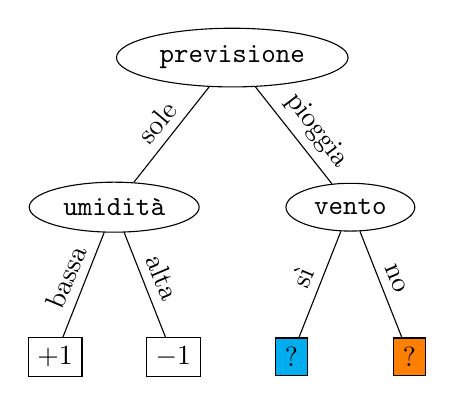
\begin{tikzpicture}[level distance=1.9cm,
    level 1/.style={sibling distance=3cm},
    level 2/.style={sibling distance=1.5cm}
]
    
    \node [ellipse,draw] {\texttt{previsione}}
        child {node[ellipse,draw] {\texttt{umidità}}
            child {node[rectangle,draw] {$+1$} edge from parent node[above,rotate=67] {bassa}}
            child {node[rectangle,draw] {$-1$} edge from parent node[above,rotate=-67] {alta}}
            edge from parent node[above,rotate=50] {sole}
        }
        child {node[ellipse,draw] {\texttt{vento}} 
            child {node[rectangle,draw,fill=cyan] {$?$} edge from parent node[above,rotate=67] {sì}}
            child {node[rectangle,draw,fill=orange] {$?$} edge from parent node[above,rotate=-67] {no}}
            edge from parent node[above,yshift=-.3em,xshift=.2em,rotate=-53] {pioggia}
        };

\end{tikzpicture}
    \captionof{figure}{Esempio di \textit{tree classifier} \quotes{in costruzione}.
    \label{fig:tree_class_ex1}}
\end{minipage}

Si prenda $\ell'$:
$$
\begin{aligned}
    &S_{\ell'} = \{ (x_3,+1),(x_4,-1),(x_6,+1),(x_8,+1),(x_9,+1) \} & N_{\ell'}=5 \\
    &S_{\ell'}^+ = \{ (x_3,+1)(x_6,+1),(x_8,+1),(x_9,+1) \} & \NlposOne=4 
        & \qquad \frac{\NlposOne}{N_{\ell'}}=\dashuline{0.8} \\
    &S_{\ell'}^- = \{ (x_4,-1) \} & \NlnegOne=1 & \qquad \frac{\NlnegOne}{N_{\ell'}}=0.2 \\
\end{aligned}
$$
L'\dashuline{ottanta percento} degli esempi che raggiungono $\ell'$ ha etichetta positiva, si può quindi
affermare che l'etichetta $y_{\ell'}=+1$.

Si prenda infine $\ell''$:
$$
\begin{aligned}
    &S_{\ell''} = \{ (x_1,+1),(x_2,-1),(x_5,-1),(x_7,-1) \} & N_{\ell''}=4 \\
    &S_{\ell''}^+ = \{ (x_1,+1) \} & \NlposTwo=1 & \qquad \frac{\NlposTwo}{N_{\ell''}}=0.25 \\
    &S_{\ell''}^- = \{ (x_2,-1),(x_5,-1),(x_7,-1) \} & \NlnegTwo=3 
        & \qquad \frac{\NlnegTwo}{N_{\ell''}}=\dashuline{0.75} \\
\end{aligned}
$$
Il \dashuline{settantacinque percento} degli esempi che raggiungono $\ell''$ ha etichetta negativa, si può quindi
affermare che l'etichetta $y_{\ell''}=-1$.